\documentclass[12pt]{article}
\usepackage{amsmath, amssymb}
\usepackage[margin=0.5cm]{geometry}
\usepackage{array}
\usepackage{helvet}
\usepackage{longtable}
\usepackage{tikz-cd}
\usepackage{tikz}
% Add libraries for positioning and arrows
\usetikzlibrary{trees, positioning, arrows}
\usepackage{changepage} % For margin adjustments

\begin{document}

\begin{center}
		{\LARGE\bfseries Special Matrices and their Properties}\par
		\vspace{1em}
\end{center}

% Matrix Type Hierarchy Tree
\begin{center}
  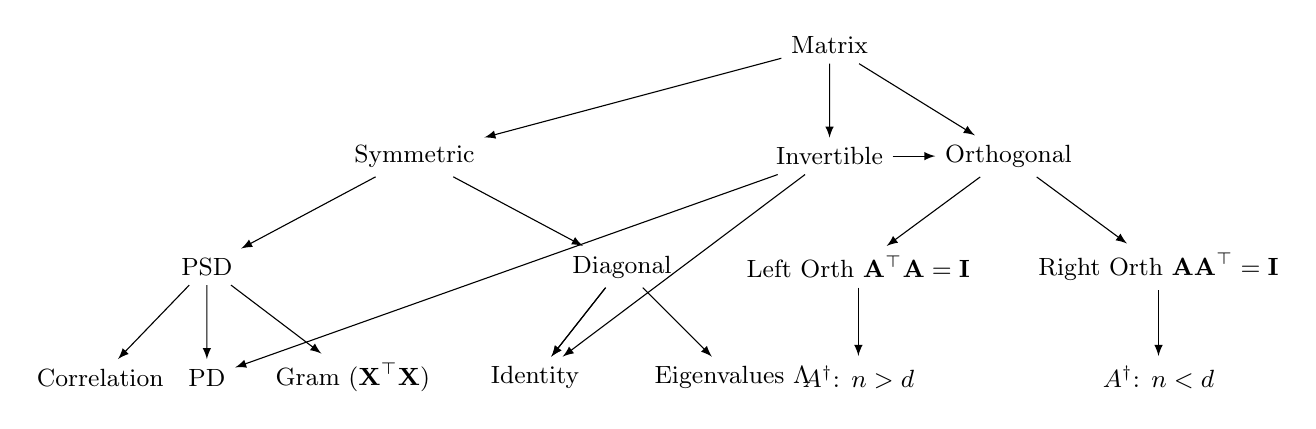
\begin{tikzpicture}[
						level distance=4em, % Adjusted level distance
						every node/.style={font=\small},
						sibling distance=15em, % Adjusted sibling distance
						edge from parent/.style={draw,-latex}
				]
    \node (Matrix) {Matrix}
				child { node (Symmetric) {Symmetric}
						child { node (PSD) {PSD} [sibling distance=3em]
								child { node [xshift=-0.3cm](Correlation) {Correlation} }
								child { node (PD) {PD} }
								child { node (Gram) [xshift=0.8cm]{Gram ($\mathbf{X}^\top\mathbf{X}$)} }
						}
						child { node (Diagonal) {Diagonal}[sibling distance=8em]
								child { node [xshift=0.3cm](Identity) {Identity} }
								child { node (EigenvalueMatrix) {Eigenvalues $\Lambda$} }
						}
				}
				child { node (Invertible) {Invertible} }
				child { node [xshift=-3cm](Orthogonal) {Orthogonal}[sibling distance=8em]
						child { node [xshift=-0.5cm](LeftOrthogonal) {Left Orth $\mathbf{A}^\top \mathbf{A}
								= \mathbf{I}$}
								child { node (Leftpseudoinverse) {$A^\dagger$: $n > d$} }
						}
						child { node [xshift=0.5cm](RightOrthogonal) {Right Orth $\mathbf{A}
								\mathbf{A}^\top = \mathbf{I}$}
								child { node (Rightpseudoinverse) {$A^\dagger$: $n < d$} }
						}
				};
				% child { node {Skew-Symmetric} }
				% child { node {Triangular} }
				% child { node {Idempotent} };
				% child { node {Nilpotent} };

    % Add arrows for overlaps
    \draw[-latex] (Invertible) -- (PD);
    \draw[-latex] (Invertible) -- (Identity);
    \draw[-latex] (Diagonal) -- (Identity);
    \draw[-latex] (Invertible) -- (Orthogonal);

  \end{tikzpicture}
  \vspace{0.5em}
\end{center}

\begin{longtable}{|>{\bfseries}m{3.5cm}|m{5cm}|m{10.5cm}|}
		\hline
		\textbf{Term} & \textbf{Definition} & \textbf{Unique Attributes /
		Key Properties} \\
		\hline
		Diagonal & $a_{ij} = 0$ for $i \ne j$ &
		- Determinant is product of diagonal entries \newline
		- Eigenvalues are diagonal entries \newline
		- $A^k$ is diagonal with entries raised to $k$ \\
		\hline
		Symmetric & $A = A^T$, i.e., $a_{ij} = a_{ji}$ &
		- All eigenvalues are real \newline
		- Eigenvectors for distinct eigenvalues are orthogonal \newline
		- Diagonalizable via orthogonal matrices \\
		\hline
		Identity ($I$) & $I_{ij} = \delta_{ij}$ &
		- $AI = IA = A$ \newline
		- $I^{-1} = I$ \newline
		- All eigenvalues are 1 \\
		\hline
		Invertible (Non-singular) & Exists $A^{-1}$ such that $AA^{-1} =
		A^{-1}A = I$ &
		- $\det(A) \ne 0$ \newline
		- Linearly independent rows and columns \newline
		- No zero eigenvalues \\
		\hline
		Singular & A square matrix with $\det(A) = 0$ &
		- Not invertible \newline
		- May have linearly dependent rows or columns \newline
		- At least one zero eigenvalue \\
		\hline
		Orthogonal & $A^{-1} = A^T$, so $A^T A = I$ &
		- Rows and columns form an orthonormal set \newline
		- Preserves lengths and angles \newline
		- $\det(A) = \pm 1$ \\
		\hline
		Left Orthogonal & $A^T A = I$ (tall matrix, $n \geq d$) &
		- Columns are orthonormal \newline
		- $A^\dagger = A^T$ (left pseudoinverse) \newline
		- Used when $A$ has full column rank \newline
		- Condition: $\text{rank}(A) = d$ where $A \in \mathbb{R}^{n \times d}$ \\
		\hline
		Right Orthogonal & $A A^T = I$ (wide matrix, $n \leq d$) &
		- Rows are orthonormal \newline
		- $A^\dagger = A^T$ (right pseudoinverse) \newline
		- Used when $A$ has full row rank \newline
		- Condition: $\text{rank}(A) = n$ where $A \in \mathbb{R}^{n \times d}$ \\

		\hline
		Pseudoinverse (Moore--Penrose) & Generalized inverse $A^\dagger$
		satisfying the four Penrose conditions &
		- Always exists and is unique for any matrix \newline
		- \textbf{Full column rank} ($n \geq d$, $\text{rank}(A) = d$): \newline
		\quad $A^\dagger = (A^T A)^{-1} A^T$ (left pseudoinverse) \newline
		- \textbf{Full row rank} ($n \leq d$, $\text{rank}(A) = n$): \newline
		\quad $A^\dagger = A^T (A A^T)^{-1}$ (right pseudoinverse) \newline
		- \textbf{Square and invertible}: $A^\dagger = A^{-1}$ \newline
		- \textbf{Rank deficient}: Computed via SVD decomposition \\

		\hline
		Positive Definite & $\vec{x}^T A \vec{x} > 0$ for all non-zero $\vec{x}$ &
		- All eigenvalues are positive \newline
		- $\det(A) > 0$ \newline
		- Invertible \\
		\hline
		Positive Semi-Definite & $A = A^T$, $\vec{x}^T A \vec{x} \ge 0$ for all $\vec{x}$ &
		- All eigenvalues are non-negative \newline
		- $\det(A) \ge 0$ \newline
		- Always symmetric \newline
		- Can always be written as $X^T X$ for some $X$ (Gram matrix) \newline
		- Defines a semi-inner product \\
		\hline
		Triangular (Upper / Lower) &
		Upper: $a_{ij} = 0$ for $i > j$; Lower: $a_{ij} = 0$ for $i < j$ &
		- Determinant is product of diagonal entries \newline
		- Eigenvalues are diagonal entries \newline
		- Solves systems efficiently via substitution \\
		\hline
		Skew-Symmetric & $A = -A^T$, so $a_{ii} = 0$ &
		- Eigenvalues are 0 or purely imaginary \newline
		- $\vec{x}^T A \vec{x} = 0$ for all $\vec{x}$ \\
		\hline
		Idempotent & $A^2 = A$ &
		- Used in projection operations \newline
		- Eigenvalues are 0 or 1 \\
		\hline
		Nilpotent & $A^k = 0$ for some $k \in \mathbb{N}$ &
		- All eigenvalues are 0 \\
		\hline
		Orthogonal Projection & Linear transformation $P$ where $P^2 = P$
		and $P = P^T$ &
		- Projects onto a subspace along its orthogonal complement \newline
		- Minimizes distance to the subspace (best approximation) \newline
		- $\text{Im}(P)$ is a subspace; $\text{Ker}(P) = \text{Im}(I - P)$ \\
		\hline
		Linear Map (Transformation) & Function $T: V \rightarrow W$
		satisfying $T(a\vec{x} + b\vec{y}) = aT(\vec{x}) + bT(\vec{y})$ &
		- Represented by a matrix in finite dimensions \newline
		- Preserves linear structure \newline
		- Kernel and image define fundamental subspaces \\
		\hline
		Fundamental Subspaces & Column space, row space, null space, left null space &
		- Column space: span of columns (range of $A$) \newline
		- Row space: span of rows = col space of $A^T$ \newline
		- Null space: solutions to $A\vec{x} = 0$ \newline
		- Left null space: null space of $A^T$ \\
		\hline
		Unitary & $U^\dagger = U^{-1}$, where $U^\dagger$ is the conjugate
		transpose of $U$ &
		- $U^\dagger U = U U^\dagger = I$ \newline
		- Preserves inner products: $\langle U\vec{x}, U\vec{y} \rangle =
		\langle \vec{x}, \vec{y} \rangle$ \newline
		- All eigenvalues lie on the unit circle: $|\lambda| = 1$ \newline
		- Generalization of orthogonal matrices to complex space \\
		\hline
		Gram Matrix & $G = X^T X$ for some matrix $X$ &
		- Always positive semi-definite \newline
		- Symmetric by construction \newline
		- Entries are inner products: $G_{ij} = \langle x_i, x_j \rangle$ \newline
		- Used in least squares and quadratic forms \\
		\hline
		Eigenvalue Matrix & Matrix with known eigenvalues $\lambda_1, \ldots, \lambda_n$ &
		- Can be diagonalized as $A = P\Lambda P^{-1}$ \newline
		- $\Lambda$ is diagonal matrix of eigenvalues \newline
		- $P$ contains corresponding eigenvectors as columns \newline
		- Powers: $A^k = P\Lambda^k P^{-1}$ \\
		\hline
		Eigenvalue Matrix ($\Lambda$) & Diagonal matrix $\Lambda = \text{diag}(\lambda_1,
		\ldots, \lambda_n)$ &
		- Contains eigenvalues on the diagonal \newline
		- Result of eigendecomposition/PCA \newline
		- $\Lambda_{ii} = \lambda_i$, $\Lambda_{ij} = 0$ for $i \neq j$ \newline
		- Used in spectral analysis and dimensionality reduction \\
		\hline
		Covariance Matrix & $\text{Cov}(X) = \frac{1}{n-1}(X - \mu)^T(X - \mu)$ &
		- Always positive semi-definite \newline
		- Symmetric by construction \newline
		- Diagonal entries are variances \newline
		- Off-diagonal entries are covariances \\
		\hline
		Correlation Matrix & Normalized covariance matrix with unit diagonal &
		- Positive semi-definite \newline
		- Symmetric with $\rho_{ii} = 1$ \newline
		- Entries satisfy $-1 \leq \rho_{ij} \leq 1$ \newline
		- Used in statistics and data analysis \\
		\hline
		Householder Matrix & $H = I - 2\frac{vv^T}{v^T v}$ for vector $v$ &
		- Symmetric and orthogonal \newline
		- $H^2 = I$ (involutory) \newline
		- Reflects vectors across hyperplane \newline
		- Used in QR decomposition \\
		\hline
		Permutation Matrix & Matrix with exactly one 1 in each row and column &
		- Orthogonal matrix \newline
		- Determinant is $\pm 1$ \newline
		- Reorders rows/columns when multiplied \newline
		- $P^T P = I$ and $P^{-1} = P^T$ \\
		\hline
		Circulant Matrix & Each row is cyclic shift of previous row &
		- Diagonalized by Discrete Fourier Transform \newline
		- Eigenvalues given by DFT of first row \newline
		- Used in signal processing \newline
		- Fast matrix-vector multiplication via FFT \\
		\hline
		Toeplitz Matrix & Constant along each diagonal: $a_{ij} = a_{i-j}$ &
		- Determined by $2n-1$ parameters \newline
		- Includes circulant matrices as special case \newline
		- Used in time series and signal processing \newline
		- Fast algorithms available for solving systems \\
		\hline
		Hankel Matrix & Constant along each anti-diagonal: $a_{ij} = a_{i+j}$ &
		- Symmetric if square \newline
		- Related to Toeplitz matrices \newline
		- Used in system identification \newline
		- Connection to moment problems \\
		\hline

\end{longtable}

\end{document}
